\section{Verification approach}%
\label{sec:daisy:motivation}

DaisyNFS is an implementation of the Network File System (NFS) API.\@ This is a
standard file-system interface, specified in RFC 1813~\cite{RFC:1813}
(specifically, this is the standard for NFS version 3, which is what DaisyNFS
implements). NFS is widely used, generally to export a file system across a
network to multiple clients, and widely supported by operating systems ---
Windows Server, macOS, and Linux each include an implementation of both an NFS
server and client.\footnote{Windows 10 and 11 can act as NFS clients but do not
include an NFS server.}

RFC 1813 is a good starting point for DaisyNFS's specification.
However, the RFC is a prose document with about 130 pages of English text,
which is unsuitable for a mathematical proof. Thus the first step is
to turn the RFC into something more precise. DaisyNFS's specification (described in
\cref{sec:daisy:nfs}) uses a
transition system defined in Dafny for this purpose, defining the behavior of
the protocol with an abstract state and transitions for each NFS operation that define
how it evolves the state and what value it returns. The
transition system allows non-determinism in the specification to give the
implementation some flexibility.

The transition system describes the abstraction of an NFS server, but what does
it mean for the \cc{daisy-nfsd} binary to implement this specification? To formalize
DaisyNFS's correctness we use the same \emph{concurrent, crash-safe refinement}
that was used in the GoTxn
specification. The server binary is a refinement of the NFS transition
system if every execution of the code --- including with concurrent operations
crashes --- has
user-visible behavior that the specification could also produce (that is, the
behavior is allowed by the specification). In DaisyNFS's specification the visible
behavior is defined to be network requests and responses.

DaisyNFS's concurrent, crash-safe refinement is a much more sophisticated property to verify
than sequential refinement. \Cref{fig:concurrent-refinement} illustrates the difference between the
concurrent and sequential simulation obligations.  For both forms of refinement, the basic proof technique is to construct a
\emph{forward simulation} from the code execution to the specification
transition system, which requires an invariant connecting their states and a
proof that shows the invariant is preserved by operations. In a sequential, non-crash
simulation, it is sufficient to show that each operation restores the invariant
when it returns since its intermediate states are invisible.
The complication in a
concurrent simulation is that the code can have many concurrent threads, each
running a different operation at the specification level. The
proof of any given operation must also show that the intermediate states satisfy the invariant, since at any
time other threads might run. Similarly, the proof of each operation's implementation must
consider interference with its execution from other threads at any time.

\begin{figure}
  \begin{subfigure}[m]{0.6\textwidth}
    \vspace{0pt}
  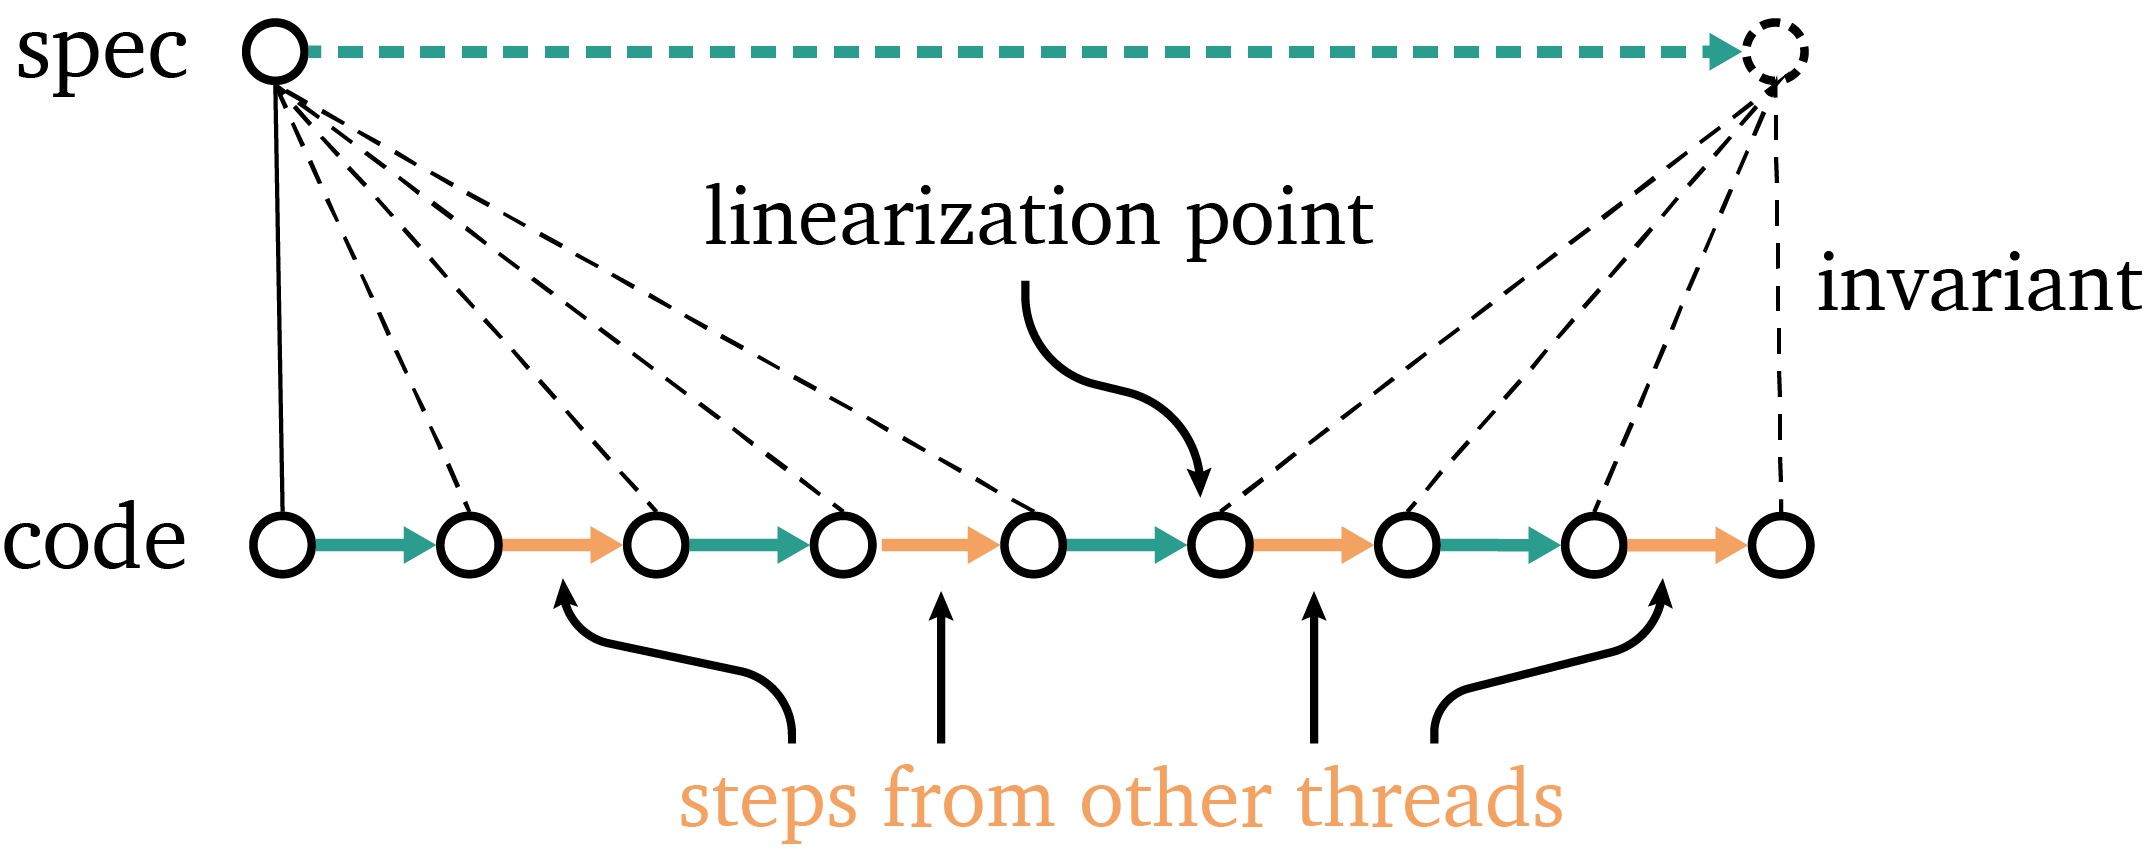
\includegraphics{fig/concurrent-refinement.png}
  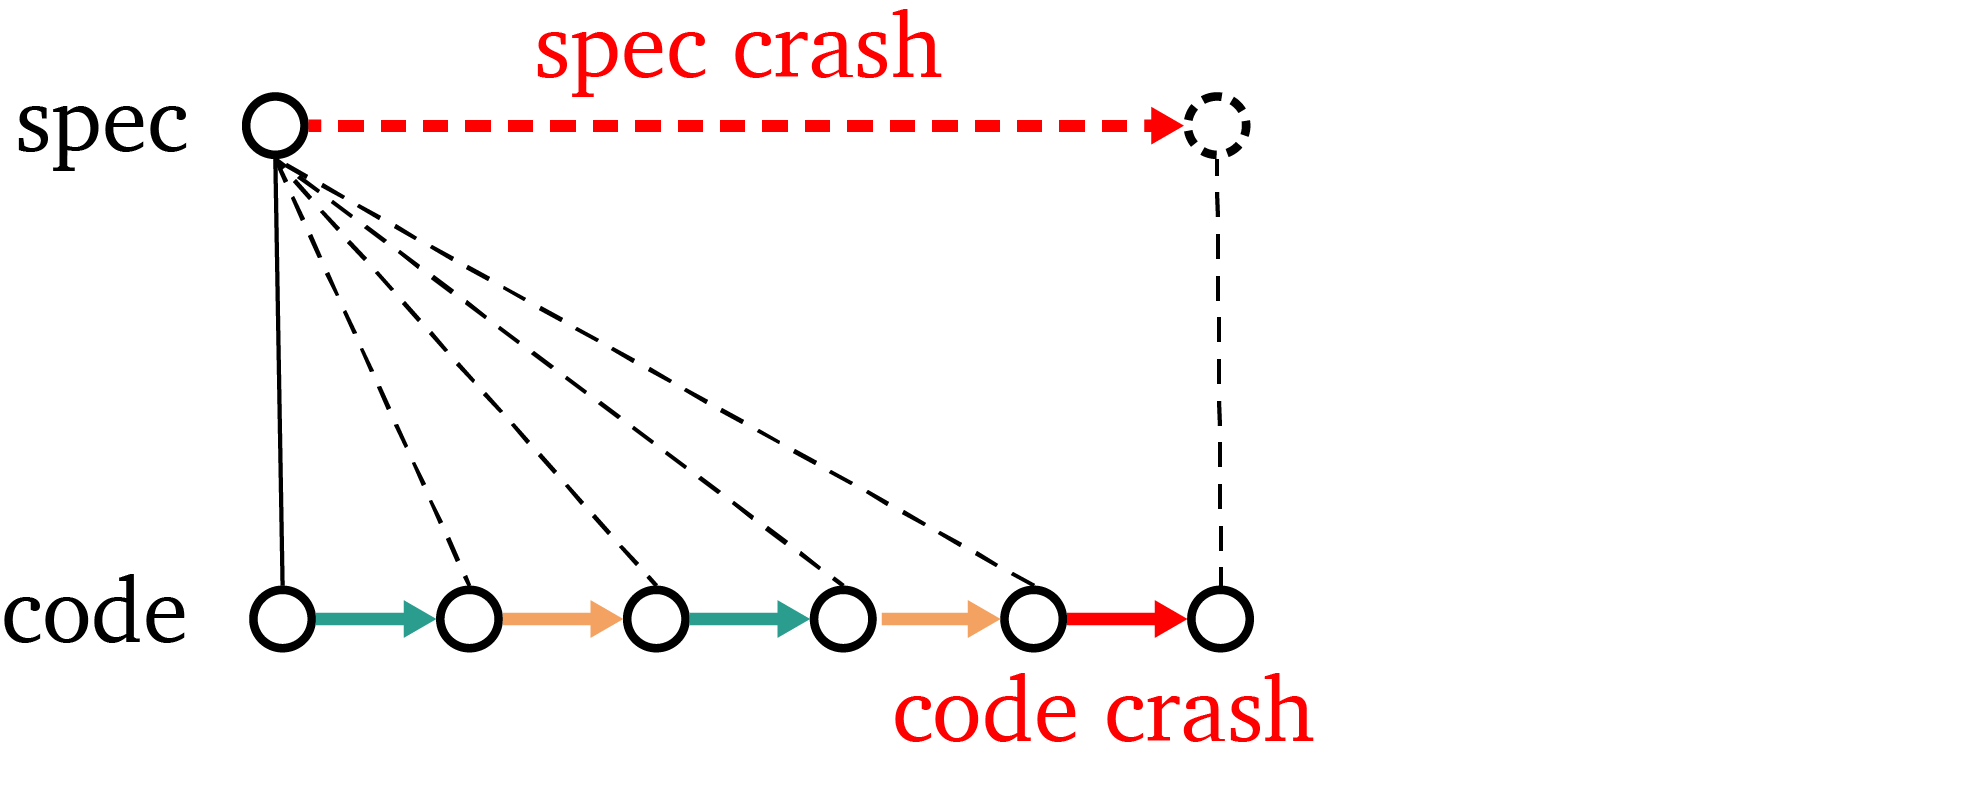
\includegraphics{fig/crash-refinement.png}
  \caption{Concurrent, crash-safe simulation}
  \label{fig:refinement:concurrent}
  \end{subfigure}%
\hfill%
  \begin{subfigure}[m]{0.4\textwidth}
    \vspace{0pt}
  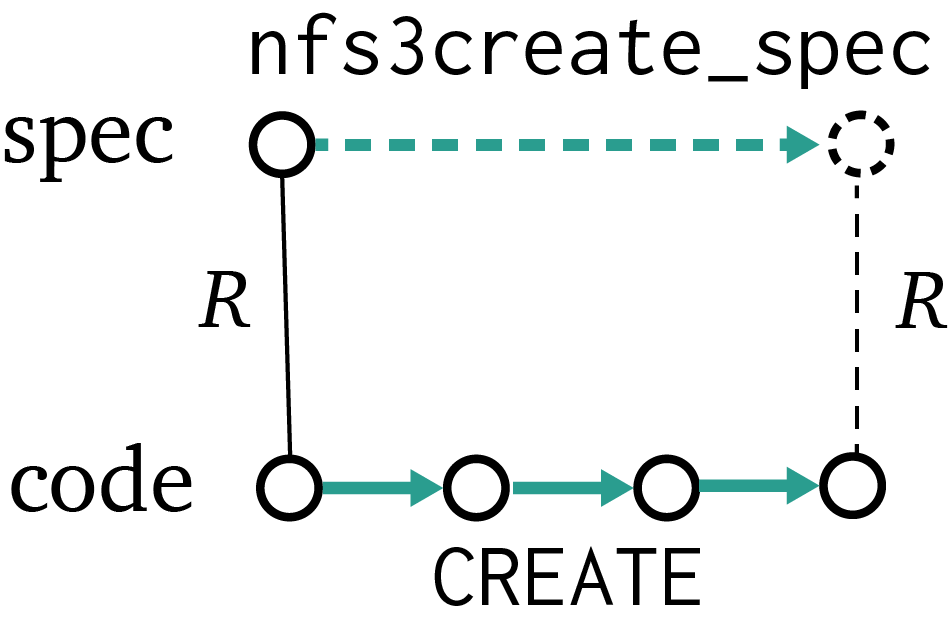
\includegraphics{fig/sequential-refinement.png}
  \caption{Sequential simulation}
  \label{fig:refinement:seq}
  \end{subfigure}
  \caption[Concurrent, crash-safe simulation vs sequential simulation]{Contrast between verifying a
    concurrent, crash-safe refinement (left) and sequential refinement (right), for a single
    procedure running the green-colored transitions. Proving concurrent
    refinement requires a proof that shows every operation (1) preserves the
    invariant at all intermediate points, and (2) simulates the abstract
    specification for the operation at some \emph{linearization point} (the
    above diagram), as well
    a similar obligation for crashes (the below diagram). For
    crash safety, a crash at any time should behave like a specification crash transition. Unlike
    sequential refinement, the proof must show the invariant holds at
    intermediate points in order to reason about potential interference with
    other threads.}

  \label{fig:concurrent-refinement}
\end{figure}


The design of DaisyNFS uses transactions, and in particular GoTxn, to simplify
the proof of concurrent refinement. Transactions appear to run
sequentially, and thus should permit reasoning about the body of each
transaction sequentially even though the actual execution interleaves multiple
transactions. This chapter describes a formalization of this intuition in the
form of a \emph{simulation-transfer theorem} (described in
\cref{sec:daisy:simulation-transfer}) which proves that a system implemented
with transactions that is verified with a sequential forward simulation against
some specification refines the same specification in the sense of a concurrent,
crash-safe refinement when run through GoTxn. The proof of this theorem is an
extension of the transaction-refinement specification from \cref{sec:txn:spec}.

Due to simulation transfer, we can use the simpler verification
methodology of sequential simulation for the DaisyNFS file-system code, compared
to the Perennial program logic used to verify the transaction system underneath.
To fully take advantage of this difference, DaisyNFS is verified using
Dafny~\cite{leino:dafny}, an entirely different tool. Dafny is a
verification-oriented programming language that is restricted to sequential
proofs. The use of Dafny greatly reduces the proof burden for verifying
DaisyNFS, because sequential proofs are well-suited to automation and Dafny's
automation is well-developed (in contrast automation for concurrent proofs is
still nascent, and would need to be integrated into Perennial to be used for
these proofs).

The value of sequential proofs can be seen in the proof-to-code ratio for the
transaction system, which is $18\times$, versus the Dafny proofs which required
about $2\times$ as many lines of proof as code. Further evidence can be seen in
the incremental development of DaisyNFS, which \cref{sec:eval:incremental}
further elaborates on.

Simulation transfer greatly reduces the proof burden for verifying DaisyNFS.
There remains the task of actually implementing the file system using
transactions. \Cref{sec:daisy:design} discusses some key challenges to address,
in particular how to ensure transactions are bounded in size (since GoTxn
transactions cannot exceed the size of the on-disk circular buffer) and avoiding
deadlocks in transactions.

\paragraph{Limitations.}
The design of DaisyNFS does impose limitations. The proof approach relies on
transactions appearing to run sequentially, which prevents modifying state
outside the transaction system. An example that would benefit from combining
the transaction system with other state is a
persistent key-value store, which needs atomic metadata updates but manages data
separately to minimize I/O --- the proof of such a system would
require explicit crash and concurrency reasoning for the data reads and writes,
but GoTxn would still be useful for managing the metadata. GoTxn does not have a
proof of liveness, and the file-system proof
does not show that transactions avoid deadlock. Our NFS implementation lacks
some features, such as symbolic links, hard links, and paginated \cc{READDIR};
we believe all of these could be implemented and specified with the same
approach but have not done so in our prototype.
